\section{Implementace vybrané části IS}\label{sec:impl}
\begingroup\sloppy

Informační systém je naprogramován v jazyce Java 21 bez frameworků a bez ORM. Desktopové rozhraní používá JavaFX, webové rozhraní běží na serveru \texttt{com.sun.net.httpserver.HttpServer} z JDK a k databázi Oracle se přistupuje přes JDBC pomocí vzoru Data Mapper. Kód je rozdělen do tří vrstev podle balíčků \texttt{presentation.\{desktop,web\}}, \texttt{business.\{domain,command,pricing,port,service\}} a \texttt{data.\{oracle,file\}}. Třída \texttt{AppContext} je místem sestavení aplikace (composition root). Načte konfigurační soubor, přes továrnu \texttt{DataAccessFactory} vytvoří datovou vrstvu a předá ji aplikačním službám. Obě uživatelská rozhraní volají jen tyto služby (vzor Facade), takže stejný případ užití se v desktopu i na webu chová stejně.

Kapitola popisuje, které případy užití jsou implementovány a jak je předvést (\odkaz{sec:impl:uc}{oddíl o případech užití}), obě uživatelská rozhraní (\odkaz{sec:impl:ui}{oddíl o rozhraních}), obě datová úložiště (\odkaz{sec:impl:storage}{oddíl o úložištích}), automatické testy (\odkaz{sec:impl:test}{oddíl o testování}) a sestavení a spuštění aplikace (\odkaz{sec:impl:run}{poslední oddíl}).

% ======================================================================
\subsection{Implementované případy užití}\label{sec:impl:uc}

Implementováno je všech 19 případů užití z \odkaz{sec:funk}{funkční specifikace}. Případy užití UC02, UC08, UC11, UC13 a UC16 jsou popsány podrobně a jsou implementovány včetně všech alternativních průběhů. \odkaz{tab:impl:uc}{Tabulka} uvádí ke každému případu užití rozhraní, ve kterém běží, třídu uživatelského rozhraní a hlavní metodu aplikační služby. Podrobně popsané případy užití jsou vyznačeny tučně.

{\small
\begin{xltabular}{\textwidth}{@{}p{1.1cm}p{1.9cm}>{\raggedright\arraybackslash}p{4.6cm}>{\raggedright\arraybackslash}X@{}}
\caption{Implementované případy užití}\label{tab:impl:uc}\\
\toprule
UC & Rozhraní & Třída UI & Metoda aplikační služby \\
\midrule
\endfirsthead
\toprule
UC & Rozhraní & Třída UI & Metoda aplikační služby \\
\midrule
\endhead
\ucref{01} & desktop, web & \texttt{LoginDialog}, \texttt{ManagerHandler} & \texttt{AuthService.loginDesktop} (desktop), \texttt{login} a \texttt{findActiveUser} (web) \\
\textbf{\ucref{02}} & desktop & \texttt{NewProjectDialog}, \texttt{MainWindow}, \texttt{UploadConflictDialog} & \texttt{ProjectService.createProject}, \texttt{DocumentService.createFolder}, \texttt{createDocument}, \texttt{downloadDocuments} \\
\ucref{03} & desktop & \texttt{EditProjectDialog} & \texttt{ProjectService.updateProject}, \texttt{archiveProject}, \texttt{reactivateProject} \\
\ucref{04} & desktop & \texttt{ProjectSearchDialog} & \texttt{ProjectService.searchProjects} \\
\ucref{05} & desktop & \texttt{CustomersWindow} & \texttt{CustomerService.search}, \texttt{create}, \texttt{update}, \texttt{delete} \\
\ucref{06} & desktop & \texttt{CatalogWindow} & \texttt{CatalogService.create}, \texttt{update}, \texttt{delete}, \texttt{findPriceHistory} \\
\ucref{07} & desktop & \texttt{MainWindow} & \texttt{MenuService.createMenu} \\
\textbf{\ucref{08}} & desktop & \texttt{MenuEditorWindow}, \texttt{MenuItemDialog} & \texttt{MenuService.openLatestRevision}, \texttt{createWorkingCopy}, \texttt{saveRevision} \\
\ucref{09} & desktop & \texttt{MenuEditorWindow} & \texttt{MenuService.listRevisions}, \texttt{openRevision} \\
\ucref{10} & desktop & \texttt{CompareRevisionsWindow} & \texttt{MenuService.compareRevisions} \\
\textbf{\ucref{11}} & desktop, web & \texttt{MenuEditorWindow}, \texttt{ShareDialog}, \texttt{MenuHandler} & \texttt{SharingService.shareRevision}, \texttt{openSharedMenu}, \texttt{addComment} \\
\ucref{12} & web & \texttt{MenuHandler}, \texttt{MenuPage} & \texttt{SharingService.openSharedMenu} \\
\textbf{\ucref{13}} & desktop & \texttt{CommentsWindow} & \texttt{SharingService.listComments}, \texttt{resolveComment} \\
\ucref{14} & desktop & \texttt{MenuEditorWindow}, \texttt{MenuPdfExport} & \texttt{MenuExportService.exportPdf} \\
\ucref{15} & web & \texttt{ManagerHandler}, \texttt{ManagerPage} & \texttt{ProjectService.searchManagedProjects}, \texttt{findManagedProject}, \texttt{loadTree}, \texttt{MenuService.openLatestRevision}, \texttt{projectIdOf} \\
\textbf{\ucref{16}} & desktop & \texttt{UsersWindow} & \texttt{UserService.createUser}, \texttt{updateUser} \\
\ucref{17} & desktop & \texttt{MainWindow}, \texttt{UsersWindow} & \texttt{UserService.findAllUsers} \\
\ucref{18} & plánovač & \texttt{ExpiredLinkScheduler} & \texttt{SharingService.deactivateExpiredLinks} \\
\ucref{19} & desktop & \texttt{MainWindow}, \texttt{DeleteDialog} & \texttt{DocumentService.deleteNodes} \\
\bottomrule
\end{xltabular}
}

Případ užití \ucref{18} nemá uživatelské rozhraní. Plánovač \texttt{ExpiredLinkScheduler} spouští deaktivaci prošlých odkazů hned po startu samostatného webového serveru (\texttt{WebMain}) a potom jednou denně. Desktopová aplikace jej spustí jen při \texttt{web.embedded=true}.

Následující postupy předvádějí podrobně popsané případy užití v běžící aplikaci. Vycházejí z testovacích dat, která naplní databázi (například projekt \uv{Svatba Novákovi} s menu \uv{Svatební menu} a \uv{Půlnoční raut}). S testovacími daty se dodávají i ukázkové účty. Role se sčítají a pravidla jsou ve třídě \texttt{AccessPolicy}. Pracovníka s rolí administrátora představuje uživatel \texttt{jzamostny}, administrátora bez role pracovníka uživatel \texttt{mkral} (po přihlášení se otevře rovnou správa uživatelů) a manažera bez dalších rolí uživatel \texttt{tsvoboda}. Manažer se do desktopové aplikace nepřihlásí a dostane odkaz na webový přehled. Ve webovém přehledu vidí jen projekty pracovníků, kteří mu podléhají. Uživatel \texttt{mkral} je zároveň manažerem uživatele \texttt{jzamostny}, a proto ve webovém přehledu vidí jeho projekty včetně projektu \uv{Svatba Novákovi}. Všechny ukázkové účty mají heslo \texttt{heslo123}, které je nutné v ostrém provozu změnit. Kontrolu stavu po ukončení případu užití lze provést dotazem SQL do uvedených tabulek. Odpovídá části \uv{Stav systému po ukončení případu užití} ve funkční specifikaci.

\subsubsection{Ukázka UC02 -- Vytvořit projekt a spravovat jeho dokumenty}

\textbf{Hlavní průběh.} V hlavním okně zvolte \uv{+ Nový projekt}, vyplňte název, vyberte zákazníka, zadejte budoucí datum akce, místo a počet hostů a zvolte \uv{Vytvořit projekt}. Nový projekt se zobrazí s prázdnou kořenovou složkou. V nabídce \uv{+ Nový} zvolte \uv{Složka} a zadejte název, například \uv{Podklady}. Vyberte novou složku ve stromu, v nabídce \uv{+ Nový} zvolte \uv{Menu} a zadejte název menu. Menu se otevře dvojklikem a pokračuje se \ucref{08}.

\textbf{Alternativní průběhy.} Neplatné údaje projektu (\odkaz{uc:02:4.1}{4.1}) předvedete zadáním počtu hostů 0 nebo data v minulosti. Formulář zvýrazní chybná pole a projekt nevznikne. Existující název (\odkaz{uc:02:6.1}{6.1} a \odkaz{uc:02:8.1}{8.1}) předvedete tak, že v projektu \uv{Svatba Novákovi} vytvoříte v kořenové složce složku \uv{Podklady} nebo menu \uv{Svatební menu}. Zobrazí se dialog \uv{Název již existuje} s předvyplněným volným názvem a volbami \uv{Přejmenovat} a \uv{Zrušit}. Nahrání dokumentu (\odkaz{uc:02:7.1}{7.1}) předvedete tlačítkem \uv{Nahrát dokument} a výběrem souboru. Soubor větší než 20~MB systém odmítne s chybovou zprávou. Pro stažení označte v obsahu složky jeden nebo více dokumentů a zvolte \uv{Stáhnout}. Tlačítko je aktivní jen tehdy, když jsou označeny pouze dokumenty.

\textbf{Kontrola úložišť.} V tabulce \texttt{projects} je nový řádek se stavem \texttt{IN\_PROGRESS}, s \texttt{customer\_id} a \texttt{responsible\_user\_id}. V tabulce \texttt{project\_nodes} jsou kořenová složka, podsložka (\texttt{node\_type = 'FOLDER'}) a menu (\texttt{'MENU'}). V tabulce \texttt{menu\_revisions} je revize 1 ve stavu \texttt{WORKING} bez řádků v \texttt{menu\_categories}. Nahraný dokument má v \texttt{project\_nodes} typ \texttt{'DOCUMENT'} a vyplněné sloupce \texttt{content\_type}, \texttt{size\_bytes} a \texttt{storage\_key}. Jeho obsah leží ve složce dokumentů v souboru \texttt{p<id projektu>/<UUID>-<název>}, tedy pod klíčem uloženým ve sloupci \texttt{storage\_key}.

\subsubsection{Ukázka UC08 -- Upravit menu a uložit revizi}

\textbf{Hlavní průběh.} Otevřete dvojklikem menu, jehož nejnovější revize je ve stavu PRACOVNÍ (v testovacích datech \uv{Svatební menu}, revize 3). Vyberte kategorii, zvolte \uv{+ Přidat položku}, vyberte produkt a zadejte množství a cenu. Množství a cenu existující položky změníte tlačítkem \uv{Upravit položku}. Panel vpravo po každé změně přepočítá cenu celkem a na hosta a tlačítko \uv{Zpět} poslední změnu vrátí. Zvolte \uv{Uložit revizi} a zadejte poznámku. Systém oznámí \uv{Uloženo jako revize č.~3} a číslo revize se nezmění.

\textbf{Alternativní průběhy.} Sdílenou revizi (\odkaz{uc:08:2.1}{2.1}) předvedete na menu \uv{Půlnoční raut}, jehož nejnovější revize 4 je SDÍLENÁ. Editor ji zobrazí jen pro čtení s upozorněním. Po volbě \uv{Vytvořit pracovní kopii} se editace povolí a uložení vytvoří revizi 5. Chyby v menu (\odkaz{uc:08:6.1}{6.1}) předvedete nastavením množství položky na 0. Systém nic neuloží, oznámí \uv{Menu obsahuje chyby a nebylo uloženo} a chybný řádek zvýrazní červeně. Souběžnou změnu (\odkaz{uc:08:7.1}{7.1}) předvedete tak, že stejné menu otevřete dvakrát a uložíte nejprve v jednom a pak ve druhém okně. Druhé uložení skončí zprávou \uv{Menu mezitím změnil jiný pracovník} a editor načte nejnovější revizi.

\textbf{Kontrola úložišť.} Řádek pracovní revize v \texttt{menu\_revisions} má novou hodnotu \texttt{note}, \texttt{created\_by} a \texttt{created\_at}. Řádky v \texttt{menu\_categories} a \texttt{menu\_items} odpovídají uloženému stavu. Při pracovní kopii je v \texttt{menu\_revisions} nový řádek s číslem o jedna vyšším ve stavu \texttt{WORKING}. Řádky sdílené revize a její odkaz v \texttt{share\_links} se nezměnily.

\subsubsection{Ukázka UC11 -- Sdílet nabídku se zákazníkem a přidat komentář}

\textbf{Hlavní průběh.} V editoru menu se uloženou revizí s alespoň jednou kategorií zvolte \uv{Sdílet se zákazníkem}. Dialog zobrazí odkaz tvaru \texttt{http://localhost:8080/menu/<token>} a QR kód. Odkaz zkopírujte tlačítkem \uv{Kopírovat} a otevřete v prohlížeči. Stránka zobrazí nabídku s cenami a alergeny a odkaz \uv{zobrazit s DPH} přepne ceny. V části \uv{Přidat komentář} vyplňte \uv{Vaše jméno}, případně vyberte položku v poli \uv{Týká se}, napište komentář a zvolte \uv{Odeslat komentář}. Stránka potvrdí \uv{Komentář byl odeslán.} a komentář se objeví v seznamu. Pracovník jej uvidí v editoru na tlačítku s počtem nevyřízených komentářů.

\textbf{Alternativní průběhy.} Nahrazený odkaz (\odkaz{uc:11:5.1}{5.1}) předvedete tak, že si první odkaz uschováte, v desktopu vytvoříte pracovní kopii, uložíte ji a sdílíte znovu. Starý odkaz pak zobrazí stránku \uv{Odkaz již není platný} s tlačítkem \uv{Zobrazit aktuální nabídku}, které vede na novou revizi. Neexistující odkaz, například s pozměněným tokenem, zobrazí zprávu \uv{Odkaz není platný, kontaktujte pracovníka.} Neplatný komentář (\odkaz{uc:11:7.1}{7.1}) předvedete odesláním formuláře s prázdným jménem. Komentář se neuloží a chybné pole se zvýrazní.

\textbf{Kontrola úložišť.} Revize má v \texttt{menu\_revisions} stav \texttt{SHARED}. V \texttt{share\_links} je nový řádek s \texttt{active = 'Y'} a \texttt{valid\_until} o 14 dní později a dřívější odkazy téhož menu mají \texttt{active = 'N'}. V \texttt{comments} je nový řádek s \texttt{resolved = 'N'}, \texttt{author\_name}, \texttt{body}, \texttt{created\_at} a u komentáře k položce s vyplněným \texttt{product\_id}.

\subsubsection{Ukázka UC13 -- Zpracovat komentáře zákazníka}

\textbf{Hlavní průběh.} V editoru menu \uv{Svatební menu} zvolte tlačítko \uv{Komentáře k rev.~2 (1 nevyřízených)}. Okno \uv{Komentáře zákazníka} ukáže nevyřízené komentáře nahoře. Vyberte komentář, zapište \uv{Poznámku k vyřízení} (nejvýše 200 znaků) a zvolte \uv{Označit jako vyřízený}. Komentář se přesune mezi vyřízené a po vyřízení posledního se zobrazí zpráva \uv{Všechny komentáře jsou vyřízeny.}

\textbf{Alternativní průběhy.} Změnu menu podle komentáře (\odkaz{uc:13:3.1}{3.1}) předvedete volbou \uv{Upravit menu podle komentáře}. Otevře se nejnovější revize se zvýrazněnou položkou, u sdílené revize jako pracovní kopie. Po uložení se okno komentářů vrátí s předvyplněnou poznámkou \uv{Upraveno v revizi č.~N}. Souběžné vyřízení (\odkaz{uc:13:4.1}{4.1}) předvedete otevřením okna komentářů ze dvou oken editoru téhož menu. Druhý pokus o vyřízení téhož komentáře skončí zprávou, kdo a kdy jej vyřídil. Předčasné ukončení (\odkaz{uc:13:7.1}{7.1}) je volba \uv{Zavřít}, po které editor dál ukazuje počet nevyřízených komentářů.

\textbf{Kontrola úložišť.} Zpracovaný komentář má v \texttt{comments} hodnoty \texttt{resolved = 'Y'}, \texttt{resolution\_note}, \texttt{resolved\_by} (identifikátor pracovníka) a \texttt{resolved\_at}. Ostatní komentáře mají stále \texttt{resolved = 'N'}. Při změně menu je v \texttt{menu\_revisions} uložená revize, jejíž číslo uvádí \texttt{resolution\_note}.

\subsubsection{Ukázka UC16 -- Spravovat uživatele a oprávnění}

\textbf{Hlavní průběh.} Přihlaste se jako \texttt{jzamostny} (pracovník a administrátor) a v hlavním okně zvolte \uv{Administrátorský režim}. Uživatel \texttt{mkral} bez role pracovníka se dostane do správy uživatelů rovnou po přihlášení. Zobrazí se okno \uv{Uživatelé a oprávnění}. Zvolte \uv{+ Nový uživatel}, vyplňte \uv{Uživatelské jméno}, \uv{Celé jméno}, \uv{E-mail}, \uv{Počáteční heslo (nejméně 8 znaků)}, zaškrtněte role a zvolte \uv{Uložit}. Potom vyberte v seznamu existujícího uživatele, změňte role, zrušte zaškrtnutí \uv{Účet je aktivní} nebo vyplňte pole \uv{Nastavit nové heslo} a zvolte \uv{Uložit}. Administrátorský režim ukončí tlačítko \uv{Ukončit režim administrátora}.

\textbf{Alternativní průběhy.} Neplatné údaje (\odkaz{uc:16:4.1}{4.1}) předvedete heslem kratším než 8 znaků nebo uživatelským jménem, které již existuje (například \texttt{tsvoboda}). Uživatel se neuloží a chyba se zobrazí u pole. Odebrání posledního administrátora (\odkaz{uc:16:7.1}{7.1}) předvedete tak, že role Administrátor odeberete uživatelům \texttt{jzamostny} a \texttt{kpokorny} a potom zkusíte odebrat i uživateli \texttt{mkral}. Systém změnu odmítne se zprávou \uv{Systém musí mít alespoň jednoho aktivního administrátora} a vrátí ve formuláři původní hodnoty.

\textbf{Kontrola úložišť.} V tabulce \texttt{users} je nový řádek s \texttt{password\_hash} (hash PBKDF2, nikoli heslo) a \texttt{active = 'Y'}. Jeho role jsou v \texttt{user\_roles} ve sloupci \texttt{role\_code}. Upravený uživatel má nové řádky v \texttt{user\_roles}, případně \texttt{active = 'N'} nebo nový \texttt{password\_hash}. Dotaz na aktivní uživatele s rolí \texttt{ADMIN} vrátí alespoň jeden řádek.

% ======================================================================
\subsection{Uživatelská rozhraní}\label{sec:impl:ui}

Systém má dvě uživatelská rozhraní nad stejnými aplikačními službami. Desktopová aplikace v JavaFX (balíček \texttt{presentation.desktop}, spouštěcí třída \texttt{DesktopApp}) slouží pracovníkům a administrátorům. Webové rozhraní (balíček \texttt{presentation.web}, třída \texttt{WebServer}) slouží zákazníkům na stránkách sdílené nabídky a manažerům v přehledu \texttt{/manager}. Stránky webu generují třídy \texttt{MenuPage} a \texttt{ManagerPage} jako čisté HTML s vloženým stylem a bez JavaScriptu. Rozhraní odpovídají \odkaz{sec:ui}{skicám uživatelského rozhraní}. Volbu cen s DPH nebo bez DPH zajišťuje v obou rozhraních vzor Strategy (\texttt{PriceStrategy}, \texttt{PriceWithVat}, \texttt{PriceWithoutVat}).

Hlavní okno (\odkaz{fig:impl:main}{obrázek}) odpovídá skice \odkaz{fig:d1}{D1}. Archivovaný projekt (\odkaz{fig:impl:archived}{obrázek}) je jen pro čtení, takže tlačítka pro změny jsou zakázána. Tlačítko \uv{Obnovit projekt} v dialogu úprav projektu jej po potvrzení vrátí do stavu rozpracovaný a změny jsou znovu povolené. Editor menu (\odkaz{fig:impl:editor}{obrázek}) odpovídá skice \odkaz{fig:d4}{D4} a okno komentářů (\odkaz{fig:impl:comments}{obrázek}) skice \odkaz{fig:d5}{D5}. Editor se před zavřením s neuloženými změnami zeptá na potvrzení a poznámka položky je označena \uv{Poznámka (vidí zákazník)}, protože ji zákazník vidí na webu. Okno komentářů má tlačítko \uv{Obnovit}. Správa uživatelů (\odkaz{fig:impl:users}{obrázek}) odpovídá skice \odkaz{fig:d7}{D7}. Další okna desktopu ukazují porovnání revizí, evidenci zákazníků a katalog produktů. Webová stránka zákazníka (\odkaz{fig:impl:web-customer}{obrázek}) odpovídá skice \odkaz{fig:w1}{W1}, stránka neplatného odkazu skice \odkaz{fig:w2}{W2}. Stránky manažera nemají v návrhu samostatnou skicu a používají stejný vzhled jako stránka zákazníka.

\clearpage
\begin{figure}[H]
  \centering
  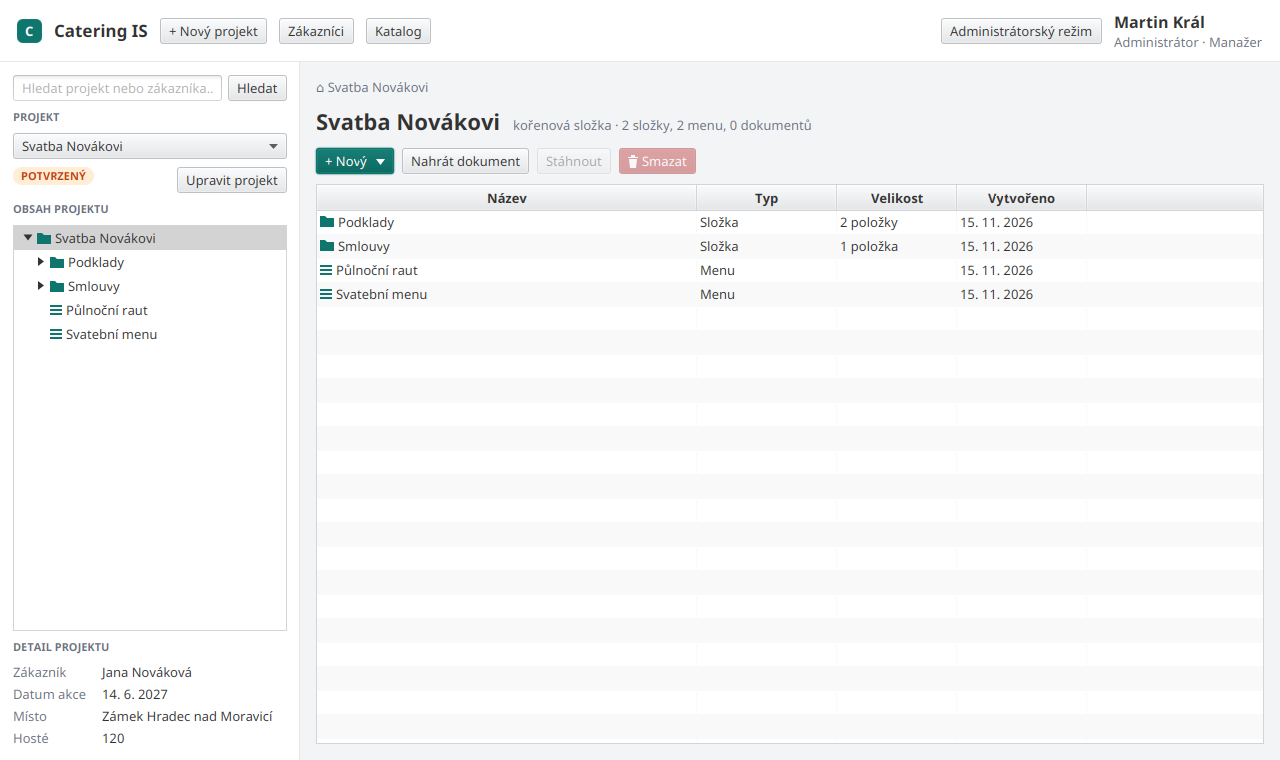
\includegraphics[width=\textwidth,height=0.38\textheight,keepaspectratio]{impl-desktop-main.png}
  \caption{Desktop -- hlavní okno s projektem \uv{Svatba Novákovi}}\label{fig:impl:main}
  \medskip
  \small Vlevo je výběr projektu, strom obsahu a detail projektu, vpravo obsah aktivní složky s tlačítky \uv{+ Nový}, \uv{Nahrát dokument}, \uv{Stáhnout} a \uv{Smazat}.
\end{figure}
\begin{figure}[H]
  \centering
  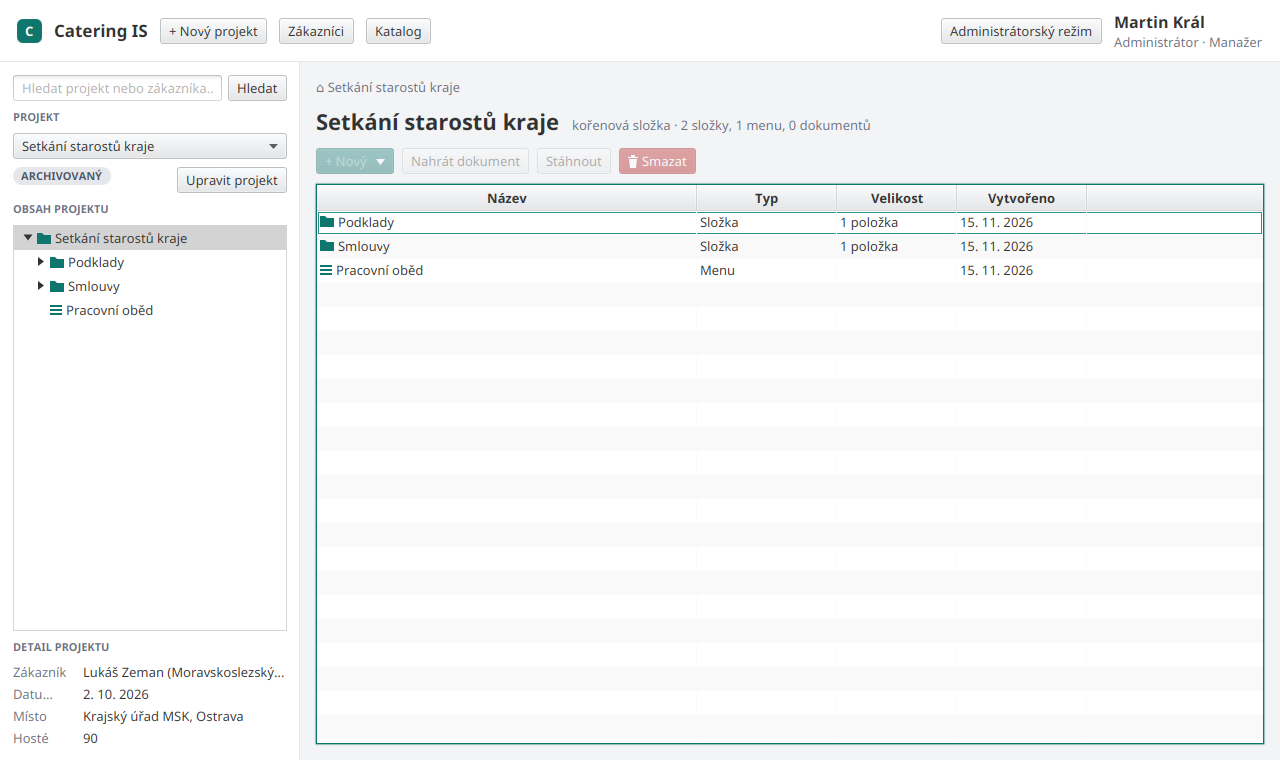
\includegraphics[width=\textwidth,height=0.38\textheight,keepaspectratio]{impl-desktop-archived.png}
  \caption{Desktop -- archivovaný projekt jen pro čtení}\label{fig:impl:archived}
  \medskip
  \small U archivovaného projektu jsou tlačítka \uv{+ Nový}, \uv{Nahrát dokument} a \uv{Smazat} zakázána.
\end{figure}
\clearpage

\begin{figure}[H]
  \centering
  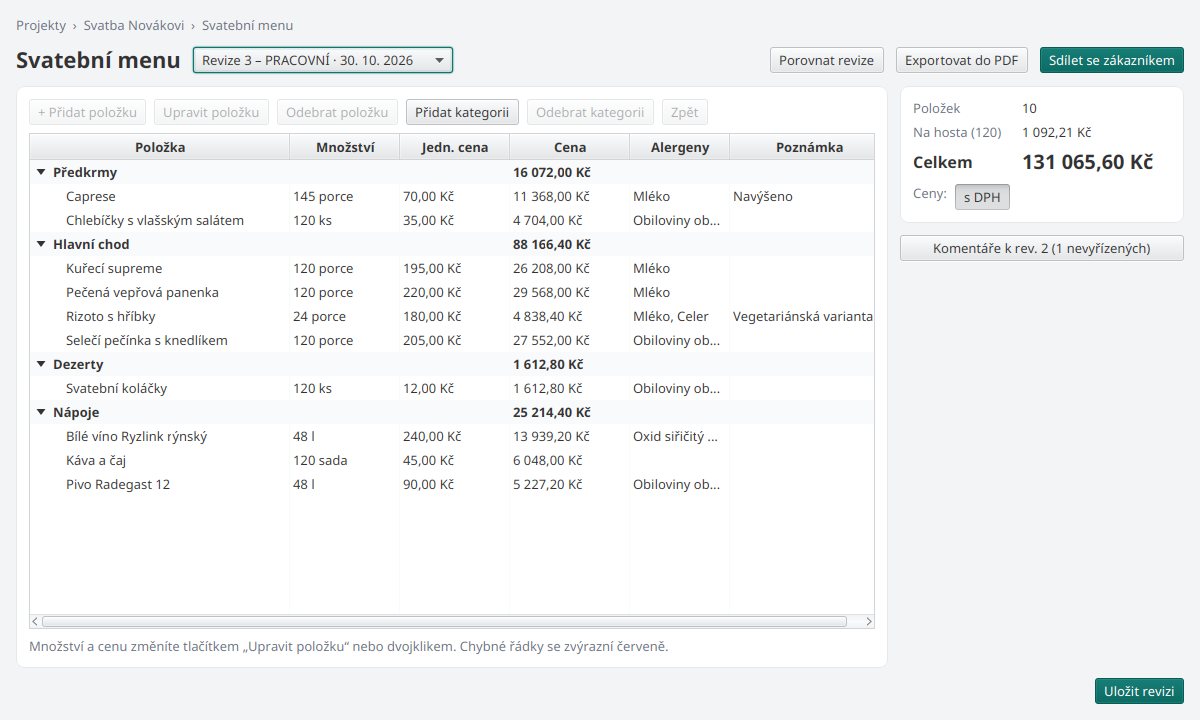
\includegraphics[width=\textwidth,height=0.38\textheight,keepaspectratio]{impl-desktop-menu-editor.png}
  \caption{Desktop -- editor menu s pracovní revizí}\label{fig:impl:editor}
  \medskip
  \small Editor ukazuje kategorie a položky revize, průběžně počítanou cenu a tlačítko s počtem nevyřízených komentářů.
\end{figure}
\begin{figure}[H]
  \centering
  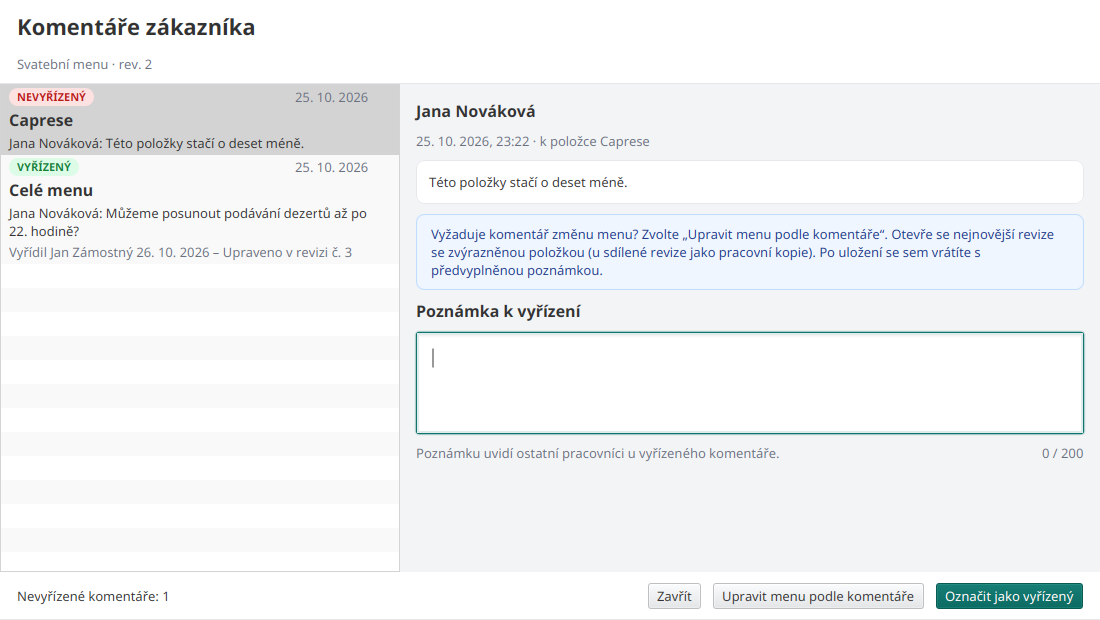
\includegraphics[width=\textwidth,height=0.38\textheight,keepaspectratio]{impl-desktop-comments.png}
  \caption{Desktop -- zpracování komentářů zákazníka}\label{fig:impl:comments}
  \medskip
  \small Nevyřízené komentáře jsou nahoře, vyřízené ukazují, kdo je vyřídil a s jakou poznámkou.
\end{figure}
\clearpage

\begin{figure}[H]
  \centering
  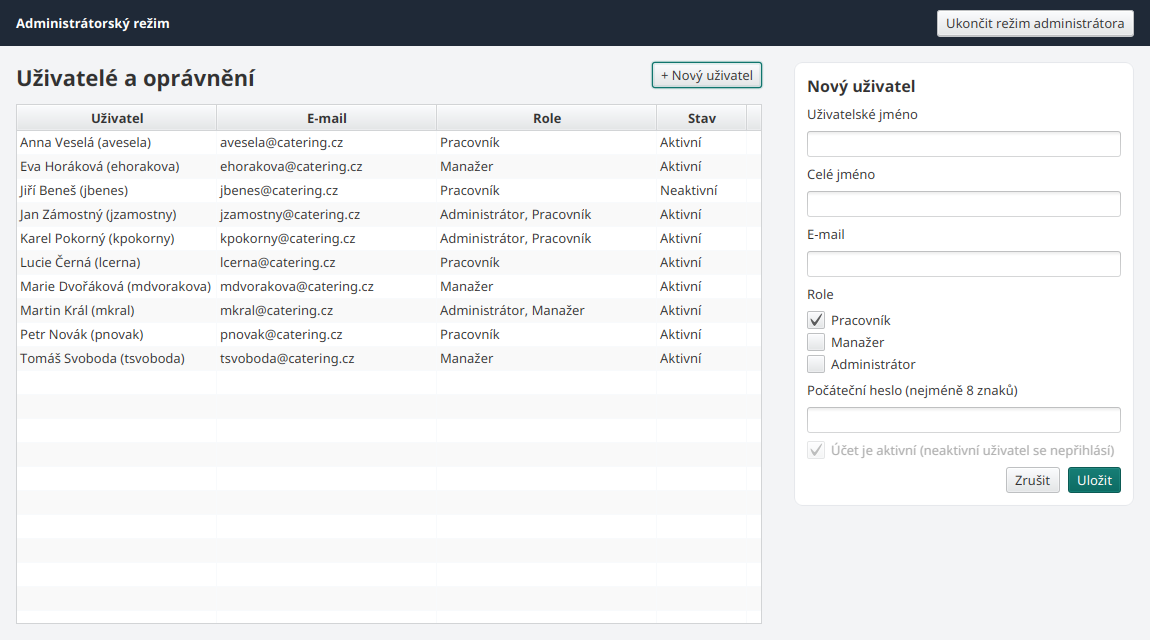
\includegraphics[width=\textwidth,height=0.38\textheight,keepaspectratio]{impl-desktop-users.png}
  \caption{Desktop -- správa uživatelů v administrátorském režimu}\label{fig:impl:users}
  \medskip
  \small Seznam uživatelů s rolemi a stavem a formulář nového uživatele.
\end{figure}
\begin{figure}[H]
  \centering
  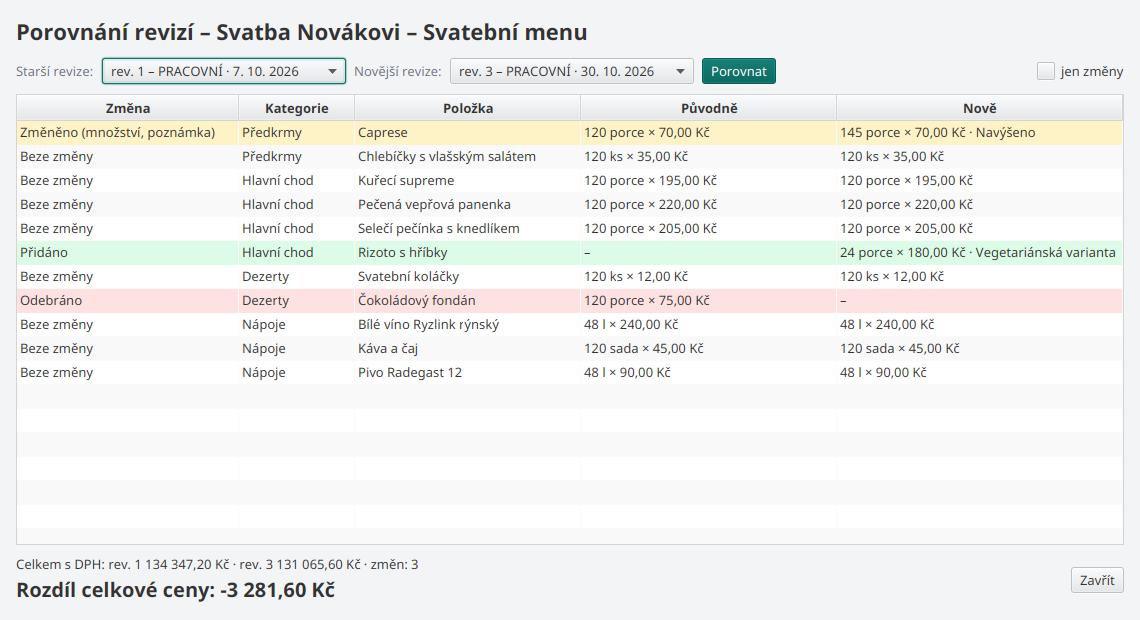
\includegraphics[width=\textwidth,height=0.38\textheight,keepaspectratio]{impl-desktop-compare.png}
  \caption{Desktop -- porovnání revizí menu}\label{fig:impl:compare}
  \medskip
  \small Přidané položky jsou zeleně, odebrané červeně a změněné žlutě, dole je rozdíl celkové ceny.
\end{figure}
\clearpage

\begin{figure}[H]
  \centering
  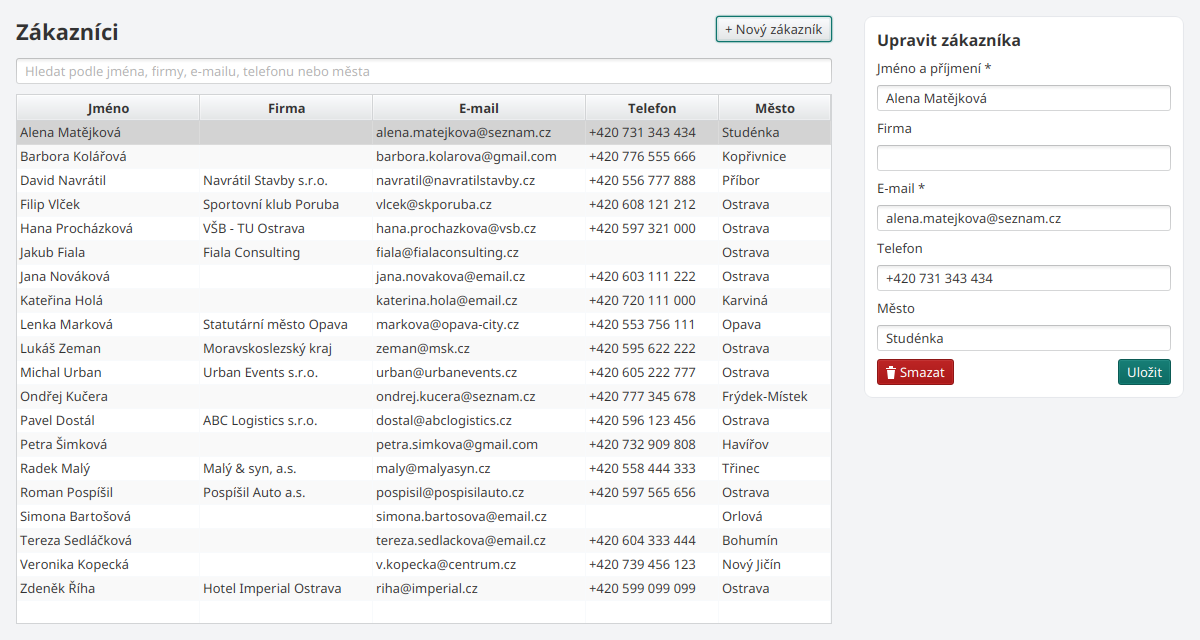
\includegraphics[width=\textwidth,height=0.38\textheight,keepaspectratio]{impl-desktop-customers.png}
  \caption{Desktop -- evidence zákazníků}\label{fig:impl:customers}
  \medskip
  \small Vyhledávání v seznamu zákazníků a formulář pro jejich vytvoření, úpravu a smazání.
\end{figure}
\begin{figure}[H]
  \centering
  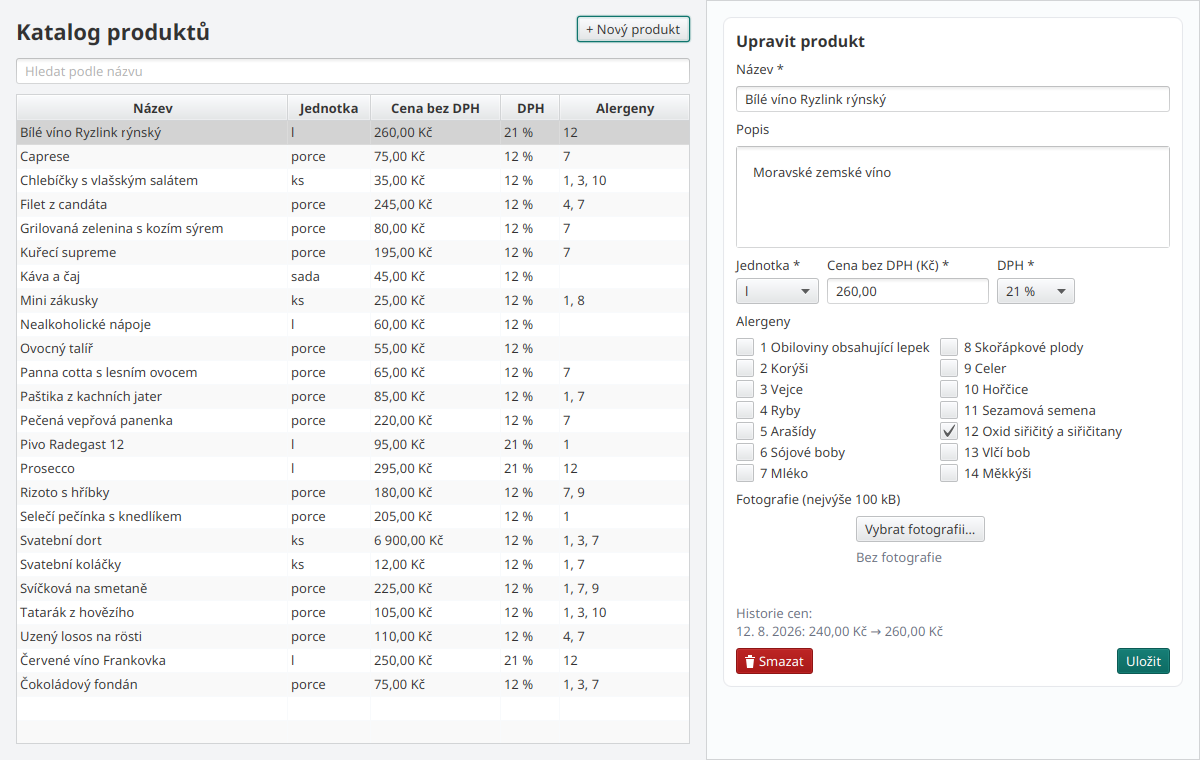
\includegraphics[width=\textwidth,height=0.38\textheight,keepaspectratio]{impl-desktop-catalog.png}
  \caption{Desktop -- katalog produktů}\label{fig:impl:catalog}
  \medskip
  \small Produkt má jednotku, cenu, sazbu DPH, alergeny, fotografii do 100~kB a historii cen.
\end{figure}
\clearpage

\begin{figure}[H]
  \centering
  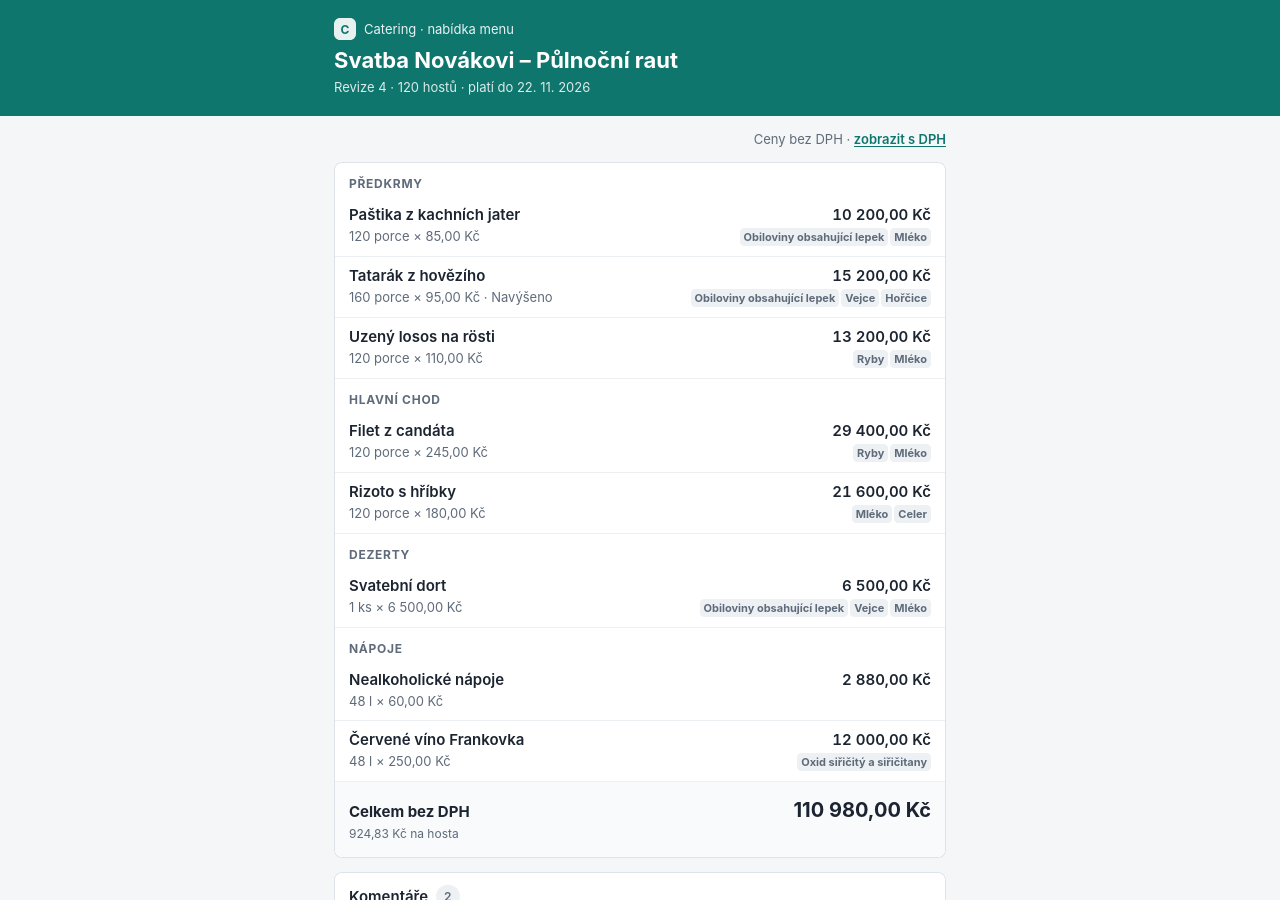
\includegraphics[width=\textwidth,height=0.38\textheight,keepaspectratio]{impl-web-customer-menu.png}
  \caption{Web -- sdílená nabídka pro zákazníka}\label{fig:impl:web-customer}
  \medskip
  \small Zákazník vidí revizi menu s cenami a alergeny, pod ní komentáře a formulář nového komentáře.
\end{figure}
\begin{figure}[H]
  \centering
  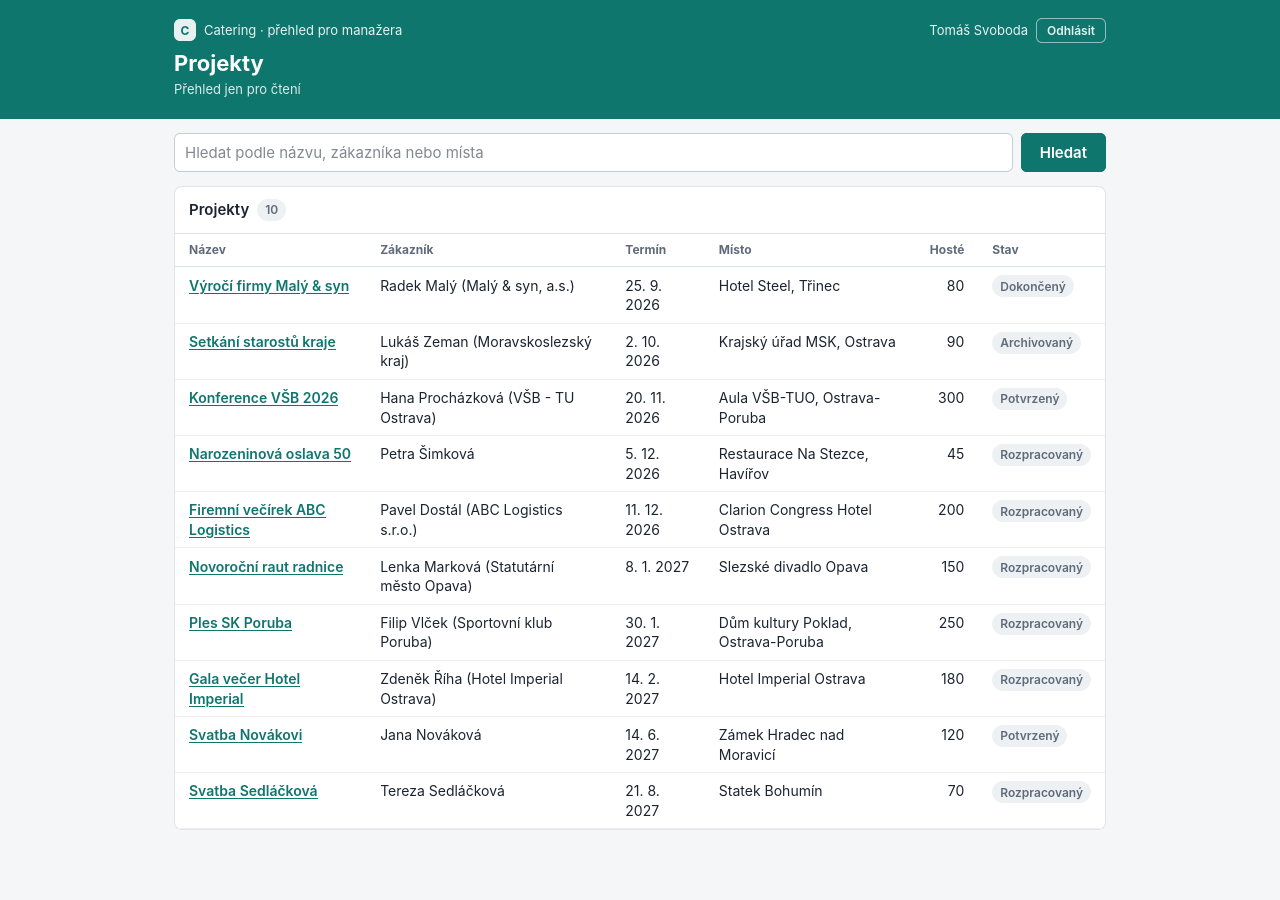
\includegraphics[width=\textwidth,height=0.38\textheight,keepaspectratio]{impl-web-manager-list.png}
  \caption{Web -- přehled projektů pro manažera}\label{fig:impl:web-list}
  \medskip
  \small Po přihlášení na adrese \texttt{/manager} vidí manažer seznam projektů s vyhledáváním, jen pro čtení.
\end{figure}
\clearpage

\begin{figure}[H]
  \centering
  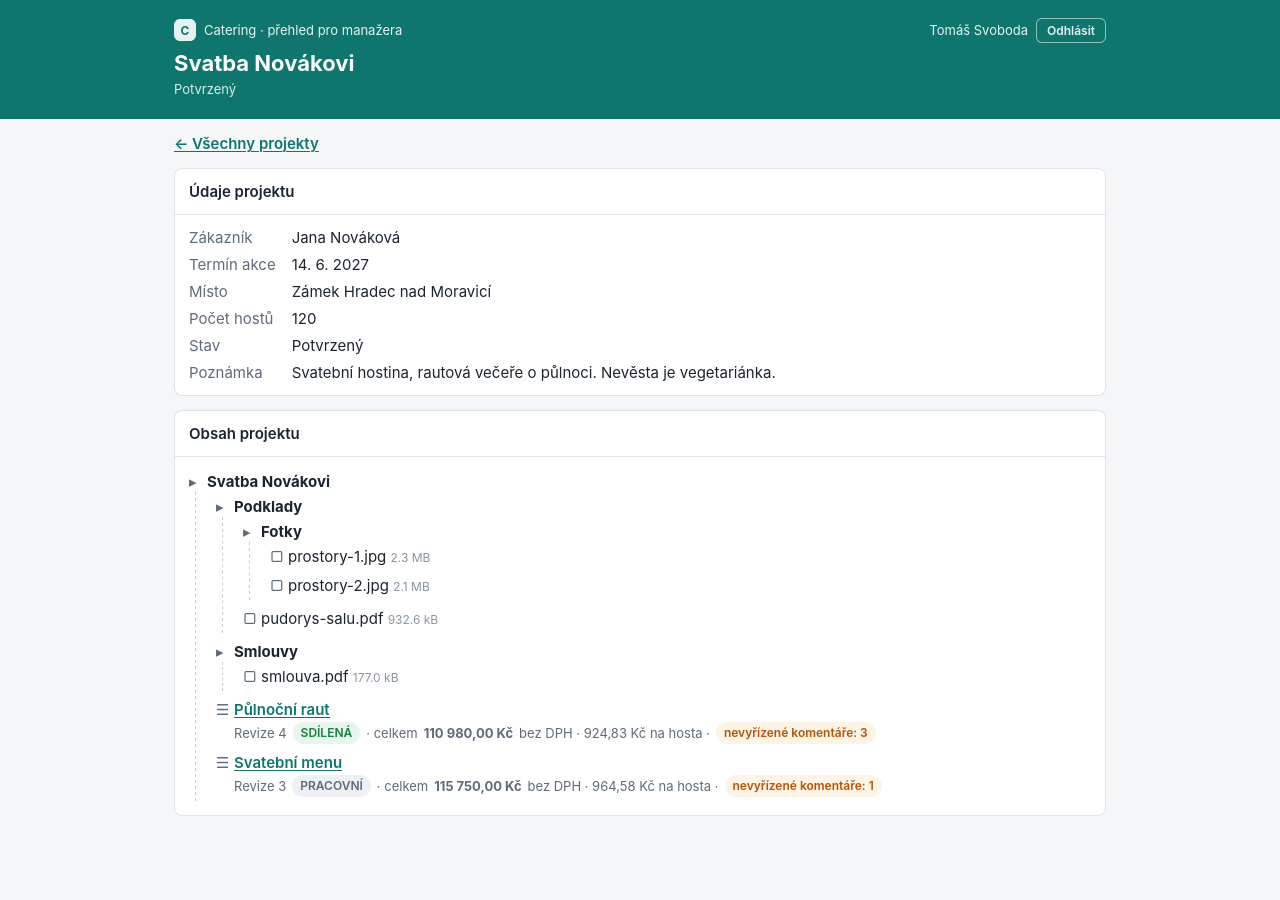
\includegraphics[width=\textwidth,height=0.38\textheight,keepaspectratio]{impl-web-manager-project.png}
  \caption{Web -- detail projektu pro manažera}\label{fig:impl:web-project}
  \medskip
  \small Údaje projektu, strom jeho obsahu a u každého menu stav nejnovější revize, cena a počet nevyřízených komentářů.
\end{figure}
\begin{figure}[H]
  \centering
  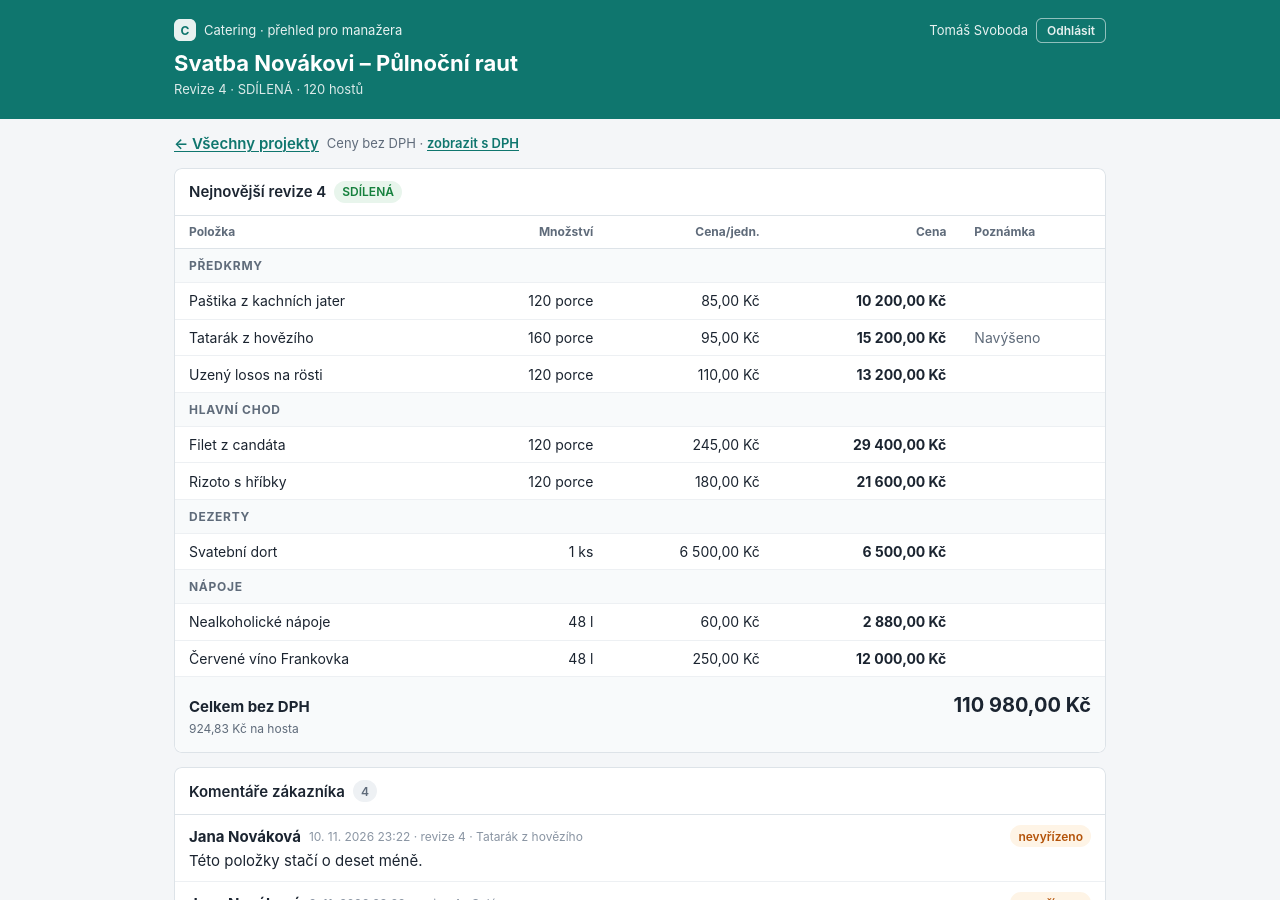
\includegraphics[width=\textwidth,height=0.38\textheight,keepaspectratio]{impl-web-manager-menu.png}
  \caption{Web -- menu projektu pro manažera}\label{fig:impl:web-menu}
  \medskip
  \small Nejnovější revize menu s cenami a se všemi komentáři zákazníka.
\end{figure}
\clearpage

% ======================================================================
\subsection{Datová úložiště}\label{sec:impl:storage}

Systém ukládá data do dvou různých úložišť podle \odkaz{sec:uloziste}{technické specifikace}. Obě jsou zpřístupněna vzory pro přístup k datům a aplikační vrstva zná jen rozhraní v balíčku \texttt{business.port}.

\begin{description}[leftmargin=0pt]
  \item[Relační databáze Oracle.] Doménové objekty ukládají datové mapovače (vzor Data Mapper) \texttt{OracleUserMapper}, \texttt{OracleCustomerMapper}, \texttt{OracleProjectMapper}, \texttt{OracleProjectNodeMapper}, \texttt{OracleMenuMapper}, \texttt{OracleShareLinkMapper} a \texttt{OracleProductMapper}. Používají jen JDBC přes pomocnou třídu \texttt{Jdbc}. Uzly projektu jsou v jedné tabulce \texttt{project\_nodes} rozlišené sloupcem \texttt{node\_type} (Single Table Inheritance). Kategorie a položky menu ukládá \texttt{OracleMenuMapper} spolu s revizí (Dependent Mapping). Transakce řídí třída \texttt{Database} (Singleton), která drží připojení probíhající transakce a implementuje port \texttt{TransactionRunner} metodou \texttt{inTransaction}. Každá metoda aplikační služby tak běží v jedné databázové transakci. Fotografie produktů jsou uloženy jako BLOB ve sloupci \texttt{products.photo} a čtou se až na vyžádání metodou \texttt{CatalogService.loadPhoto}.
  \item[Složka dokumentů na disku.] Obsah nahraných dokumentů a exportovaných PDF ukládá brána (vzor Gateway) s rozhraním \texttt{DocumentStorage} a implementací \texttt{FileDocumentStorage}. Ta ukládá soubory do složky z klíče \texttt{documents.dir} pod klíčem tvaru \texttt{p<id projektu>/<UUID>-<název>}. V databázi zůstávají jen metadata dokumentu (název, typ, velikost a klíč \texttt{storage\_key} v tabulce \texttt{project\_nodes}). V testech nahrazuje bránu Service Stub \texttt{InMemoryDocumentStorage}, který drží soubory v paměti.
\end{description}

\begin{table}[H]
  \centering
  \small
  \caption{Co je uloženo ve kterém úložišti}\label{tab:impl:storage}
  \begin{tabularx}{\textwidth}{@{}lX@{}}
    \toprule
    Úložiště & Data \\
    \midrule
    Oracle & uživatelé a role, zákazníci, projekty, strom obsahu projektu (složky, menu, metadata dokumentů), menu, revize, kategorie a položky, sdílené odkazy, komentáře, katalog produktů s alergeny, historií cen a fotografiemi \\
    Složka dokumentů & obsah nahraných dokumentů (smlouvy, půdorysy, fotografie prostor) a PDF exportovaných menu \\
    \bottomrule
  \end{tabularx}
\end{table}

Úložiště se nevolí přepínačem v konfiguraci. Volba je dána návrhem. Aplikační služby dostávají v konstruktoru jen rozhraní z \texttt{business.port} (\texttt{ProjectMapper}, \texttt{MenuMapper}, \texttt{DocumentStorage} a další) a konkrétní implementace vytváří jediné místo, továrna \texttt{DataAccessFactory}. Z konfiguračního souboru se čtou jen přístupové údaje k databázi a cesta ke složce dokumentů. Testy dosazují do týchž služeb vlastní implementace portů (falešné mapovače v paměti a \texttt{InMemoryDocumentStorage}), čímž ověřují, že aplikační vrstva na konkrétním úložišti nezávisí.

% ======================================================================
\subsection{Testování}\label{sec:impl:test}

Aplikace má 330 automatických testů v JUnit 5 ve složce \texttt{src/test}. Příkaz \texttt{mvn clean test} je spustí a všechny projdou. Testy pracující s databází si vytvářejí vlastní data a po sobě je smažou, takže databáze zůstane ve stavu testovacích dat. Testy desktopového rozhraní potřebují grafický displej. Bez něj se přeskočí.

\begin{table}[H]
  \centering
  \small
  \caption{Skupiny automatických testů}\label{tab:impl:tests}
  \begin{tabularx}{\textwidth}{@{}>{\raggedright\arraybackslash}p{4cm}>{\raggedright\arraybackslash}Xr@{}}
    \toprule
    Skupina & Co ověřuje & Testů \\
    \midrule
    Jednotkové testy aplikační vrstvy & doménové třídy, příkazy editoru menu a aplikační služby nad falešnými mapovači v paměti (\texttt{business.fake}) a nad \texttt{InMemoryDocumentStorage}, bez databáze. Patří sem i tabulka rolí (\texttt{RoleMatrixTest}) & 190 \\
    Jednotkové testy ostatních tříd & \texttt{FileDocumentStorage} nad dočasnou složkou, \texttt{PdfMenuRenderer}, \texttt{QrCode}, \texttt{ExpiredLinkScheduler} a čtení konfigurace (\texttt{AppContextTest}) & 17 \\
    Testy mapovačů Oracle & \texttt{OracleMenuMapper}, \texttt{OracleProjectNodeMapper} a \texttt{OracleUserMapper} proti skutečné databázi & 13 \\
    Testy případů užití & hlavní i alternativní průběhy případů užití nad Oracle a složkou dokumentů (balíček \texttt{business.e2e}). Stav po ukončení ověřují dotazem SQL & 55 \\
    Testy webového rozhraní & stránky zákazníka a manažera přes skutečné požadavky HTTP (\texttt{WebServerTest}, \texttt{ManagerWebTest}) včetně bezpečnostních hlaviček, omezení pokusů o přihlášení a filtrování projektů manažera & 24 \\
    Testy desktopového rozhraní & skutečná okna JavaFX ovládaná z testu (\texttt{DesktopFlowTest}, \texttt{DesktopRolesTest}, \texttt{DesktopFixesTest}, \texttt{UsersWindowTest} a další) & 31 \\
    \midrule
    Celkem & & 330 \\
    \bottomrule
  \end{tabularx}
\end{table}

Testy případů užití mají v názvu číslo kroku alternativního průběhu, například \texttt{alt71TwoEditorsOfSameWorkingRevisionSecondSaveGetsConflict} pro \ucref{08} nebo \texttt{alt71LastActiveAdministratorCannotBeRemoved} pro \ucref{16}. Ověřují tak i průběhy, které se ručně předvádějí obtížně.

% ======================================================================
\subsection{Sestavení a spuštění}\label{sec:impl:run}

Rozmístění aplikace na uzly a postup instalace popisuje \odkaz{sec:arch:instalace}{instalace v architektuře systému}. Tento oddíl shrnuje, co je potřeba k sestavení a spuštění ze zdrojových kódů.

\textbf{Požadavky.} JDK 21 nebo novější, Maven 3.9 a databáze Oracle s vytvořeným schématem a testovacími daty. Ostatní knihovny (JavaFX 21, ovladač \texttt{ojdbc11}, ZXing pro QR kód, PDFBox pro export do PDF a JUnit 5) stáhne Maven podle souboru \texttt{pom.xml}.

\textbf{Konfigurace.} Soubor \texttt{config/db.properties} vznikne zkopírováním šablony \texttt{config/db.properties.example} a vyplněním hodnot. Obsahuje tyto klíče:

\begin{itemize}[itemsep=0pt]
  \item \texttt{db.url}: adresa JDBC databáze, například\newline \texttt{jdbc:oracle:thin:@//localhost:1521/FREEPDB1},
  \item \texttt{db.user} a \texttt{db.password}: uživatel a heslo databázového schématu,
  \item \texttt{documents.dir}: složka úložiště dokumentů (výchozí \texttt{./documents}),
  \item \texttt{web.port}: port webového rozhraní (výchozí 8080),
  \item \texttt{web.embedded}: zda desktopová aplikace spustí i webový server a denní zneplatnění odkazů (výchozí \texttt{false}, pro předvedení na jednom počítači \texttt{true}),
  \item \texttt{web.baseUrl}: začátek adresy ve sdílených odkazech (výchozí \texttt{http://localhost:8080}).
\end{itemize}

\textbf{Příkazy.} Spouštějí se ve složce aplikace.

\begin{tabularx}{\textwidth}{@{}l>{\raggedright\arraybackslash}X@{}}
  \texttt{mvn clean test} & přeloží aplikaci a spustí všechny testy \\
  \texttt{mvn javafx:run} & spustí desktopovou aplikaci (\texttt{DesktopApp}). Při \texttt{web.embedded=true} spustí i webový server \\
  \texttt{mvn exec:java} & spustí jen webový server (\texttt{WebMain}) bez desktopu \\
\end{tabularx}

\textbf{Adresy webu.} Zákazník otevírá sdílenou nabídku na adrese \texttt{http://localhost:8080/menu/<token>}, kterou zobrazí dialog sdílení. Manažer se přihlašuje na adrese \texttt{http://localhost:8080/manager}. V nasazení je tato adresa dostupná jen z firemní sítě, z internetu reverzní proxy propouští pouze \texttt{/menu/}.

\textbf{Odevzdaný archiv.} Archiv ZIP obsahuje složku \texttt{src} se zdrojovými kódy a testy, soubor \texttt{pom.xml}, šablonu \texttt{config/db.properties.example} a složku \texttt{db} se skripty databáze (\texttt{01\_schema.sql}, potom \texttt{02\_seed.sql}). Neobsahuje složku \texttt{target} s výsledky překladu ani skutečný soubor \texttt{config/db.properties} s přístupovými údaji.
\endgroup
